% !TeX program = pdflatex
\documentclass[aspectratio=169, 12pt]{beamer}

% ── Packages ──────────────────────────────────────────────────────
\usepackage[T1]{fontenc}
\usepackage{charter}               % serif font matching Uni Basel style
\usepackage{amsmath,amssymb}
\usepackage{graphicx}
\usepackage{booktabs}
\usepackage{tikz}
\usepackage{xcolor}

% ── Uni Basel colours ─────────────────────────────────────────────
\definecolor{unibaselteal}{RGB}{160,196,184}   % title‐slide / section bg
\definecolor{unibaselgray}{RGB}{80,80,80}

% ── Beamer theme — clean / minimal ───────────────────────────────
\usetheme{default}
\usecolortheme{default}
\setbeamercolor{frametitle}{fg=black}
\setbeamercolor{normal text}{fg=black, bg=white}
\setbeamercolor{itemize item}{fg=black}
\setbeamercolor{itemize subitem}{fg=unibaselgray}
\setbeamerfont{frametitle}{series=\bfseries, size=\Large}
\setbeamerfont{title}{series=\bfseries, size=\Huge}
\setbeamertemplate{navigation symbols}{}       % no nav icons
\setbeamertemplate{footline}{%                 % thin black rule
  \hspace{0.03\paperwidth}%
  \rule{0.94\paperwidth}{0.4pt}\vskip4pt%
}
\setbeamertemplate{itemize items}[circle]

% ── Section‐divider slide (teal bg, centred title) ───────────────
\AtBeginSection[]{%
  \begingroup
  \setbeamercolor{background canvas}{bg=unibaselteal}
  \setbeamertemplate{footline}{\hspace{0.03\paperwidth}\rule{0.94\paperwidth}{0.4pt}\vskip4pt}
  \begin{frame}[plain,c]
    \centering
    {\usebeamerfont{title}\color{black}\insertsectionhead\par}
  \end{frame}
  \endgroup
}

% ── Title‐page template (teal background) ────────────────────────
\defbeamertemplate*{title page}{custom}[1][]{%
  \vskip1.5cm
  {\usebeamerfont{title}\usebeamercolor[fg]{title}\inserttitle\par}%
  \vskip0.6cm
  {\large\insertsubtitle\par}%
  \vfill
  {\itshape\insertauthor\par}%
  {\insertdate\par}%
}

% ── Figures path ──────────────────────────────────────────────────
\graphicspath{{../figures/}}

% ── Metadata ──────────────────────────────────────────────────────
\title{Adaptive Algorithms}
\subtitle{Continuous Optimization --- Project Presentation}
\author{Erion Krasniqi, Denis Mustafa Xhabrahimi}
\date{20/05/2026}

% ==================================================================
\begin{document}

% ── Title slide ───────────────────────────────────────────────────
{
\setbeamercolor{background canvas}{bg=unibaselteal}
\begin{frame}[plain]
  \vspace{0.5cm}
  \titlepage
\end{frame}
}

% ── Outline ───────────────────────────────────────────────────────
\begin{frame}{Outline}
\begin{enumerate}
  \setlength{\itemsep}{0.6cm}
  \item \textbf{Introduction:} Motivation \& Goal \hfill\textit{$\sim$5 min}
  \item \textbf{Related Work:} SGD, Adagrad, RMSprop, Adam \hfill\textit{$\sim$5 min}
  \item \textbf{Methodology \& Results} \hfill\textit{$\sim$5 min}
\end{enumerate}
\end{frame}

% ==================================================================
\section{Introduction}
% ==================================================================

\begin{frame}{Why Adaptive Step Sizes?}
\begin{itemize}
  \setlength{\itemsep}{0.5cm}
  \item Gradient descent: $w_{t+1} = w_t - \eta\, \nabla f(w_t)$
  \item Fixed step size $\eta$ --- one size does \textbf{not} fit all
  \item Too large $\to$ divergence; too small $\to$ slow convergence
  \item \textbf{Key idea:} let the algorithm \emph{choose} $\eta_t$ based on the observed gradient history
\end{itemize}
\end{frame}

\begin{frame}{Project Goal}
\begin{itemize}
  \setlength{\itemsep}{0.3cm}
  \item Survey adaptive first-order methods:
        \textbf{Adagrad}, \textbf{AdaGrad-Norm}, \textbf{RMSprop}, \textbf{Adam}
  \item Compare against vanilla \textbf{SGD} (baseline)
  \item Two datasets: \textbf{A9a} (binary) and \textbf{MNIST} (multi-class)
  \item Two losses: convex logistic + non-convex regularizer
\end{itemize}
\vskip0.2cm
\centering
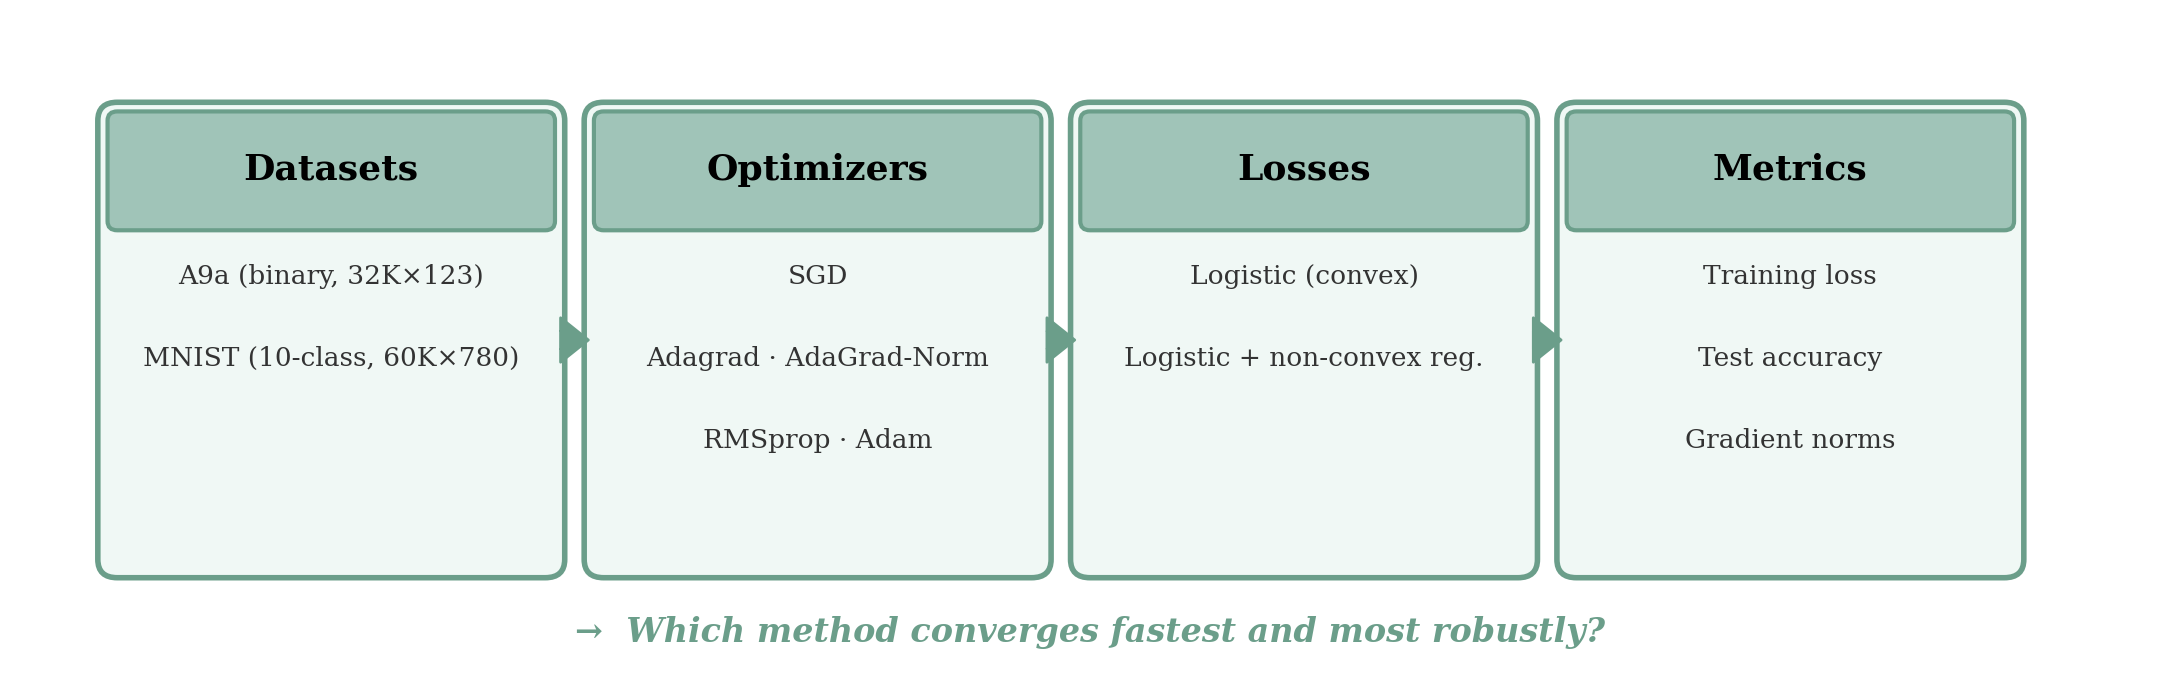
\includegraphics[width=0.85\textwidth]{visual_pipeline.png}
\end{frame}

% ==================================================================
\section{Related Work}
% ==================================================================

\begin{frame}{SGD --- Stochastic Gradient Descent}
\begin{itemize}
  \setlength{\itemsep}{0.5cm}
  \item Update: $w_{t+1} = w_t - \eta\, g_t$\,,\quad $g_t = \nabla f_{i_t}(w_t)$
  \item Simple, well-understood convergence: $\mathcal{O}(1/\sqrt{T})$
  \item Requires \textbf{careful tuning} of $\eta$
  \item No per-coordinate adaptation
\end{itemize}
\end{frame}

\begin{frame}{Adagrad \small(Duchi, Hazan \& Singer, 2011)}
\begin{itemize}
  \setlength{\itemsep}{0.4cm}
  \item Accumulate squared gradients: $G_t = G_{t-1} + g_t \odot g_t$
  \item Update: $w_{t+1} = w_t - \dfrac{\eta}{\sqrt{G_t} + \varepsilon}\, g_t$
  \item[\color{green!60!black}\textbf{+}] Per-coordinate scaling --- great for sparse features
  \item[\color{red!70!black}\textbf{--}] Step size \textbf{monotonically decreases} $\to$ can stop learning
\end{itemize}
\end{frame}

\begin{frame}{AdaGrad-Norm \small(Ward, Wu \& Bottou, 2020)}
\begin{itemize}
  \setlength{\itemsep}{0.4cm}
  \item Scalar accumulator: $b_t^2 = b_{t-1}^2 + \|g_t\|^2$
  \item Update: $w_{t+1} = w_t - \dfrac{\eta}{b_t + \varepsilon}\, g_t$
  \item[\color{green!60!black}\textbf{+}] Sharp $\mathcal{O}(1/\sqrt{T})$ convergence even on \textbf{non-convex} landscapes
  \item[\color{red!70!black}\textbf{--}] No per-coordinate adaptation (single scalar)
\end{itemize}
\end{frame}

\begin{frame}{RMSprop \small(Tieleman \& Hinton, 2012)}
\begin{itemize}
  \setlength{\itemsep}{0.4cm}
  \item Exponential moving average: $v_t = \rho\, v_{t-1} + (1-\rho)\, g_t^2$
  \item Update: $w_{t+1} = w_t - \dfrac{\eta}{\sqrt{v_t} + \varepsilon}\, g_t$
  \item[\color{green!60!black}\textbf{+}] \textbf{Forgets} old gradients $\to$ adapts faster than Adagrad
  \item[\color{green!60!black}\textbf{+}] Very fast convergence in practice
  \item[\color{red!70!black}\textbf{--}] No bias correction, no momentum
\end{itemize}
\end{frame}

\begin{frame}{Adam \small(Kingma \& Ba, 2014)}
\begin{itemize}
  \setlength{\itemsep}{0.35cm}
  \item First moment: $m_t = \beta_1 m_{t-1} + (1-\beta_1) g_t$
  \item Second moment: $v_t = \beta_2 v_{t-1} + (1-\beta_2) g_t^2$
  \item Bias correction: $\hat{m}_t = \frac{m_t}{1-\beta_1^t}$\,,\quad $\hat{v}_t = \frac{v_t}{1-\beta_2^t}$
  \item Update: $w_{t+1} = w_t - \dfrac{\eta\, \hat{m}_t}{\sqrt{\hat{v}_t} + \varepsilon}$
  \item[\color{green!60!black}\textbf{+}] Combines momentum + adaptive step size
  \item[\color{red!70!black}\textbf{--}] May not converge to optimal solution (Reddi et al.\ 2018)
\end{itemize}
\end{frame}

\begin{frame}{How the Methods Relate}
\centering
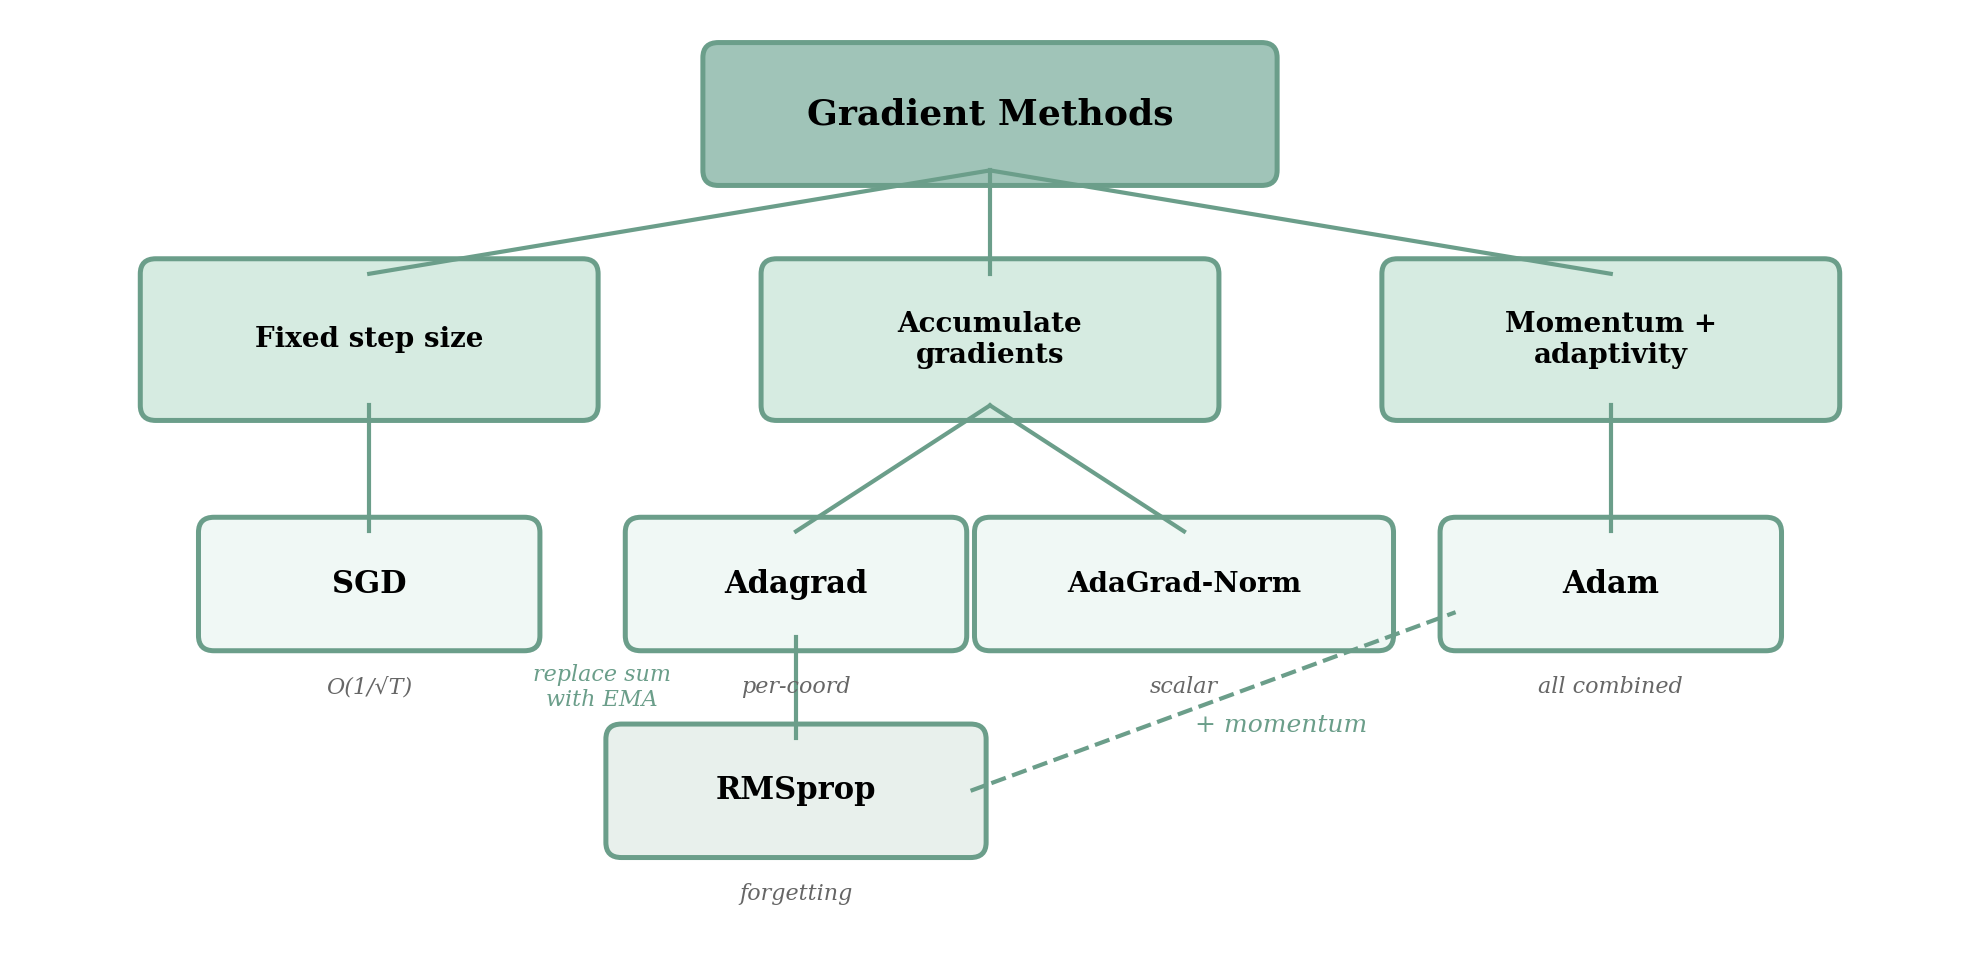
\includegraphics[width=0.72\textwidth]{visual_optimizer_tree.png}
\end{frame}

\begin{frame}{Comparison at a Glance}
\centering
\small
\begin{tabular}{@{}l c c c c@{}}
\toprule
& \textbf{Per-coord} & \textbf{Momentum} & \textbf{Forgetting} & \textbf{Convergence} \\
\midrule
SGD            & \texttimes & \texttimes & --- & $\mathcal{O}(1/\sqrt{T})$ \\
Adagrad        & \checkmark & \texttimes & \texttimes & $\mathcal{O}(\log T/\sqrt{T})$ \\
AdaGrad-Norm   & \texttimes & \texttimes & \texttimes & $\mathcal{O}(1/\sqrt{T})$ \\
RMSprop        & \checkmark & \texttimes & \checkmark & heuristic \\
Adam           & \checkmark & \checkmark & \checkmark & $\mathcal{O}(1/\sqrt{T})^*$ \\
\bottomrule
\end{tabular}

\vskip0.5cm
{\footnotesize $^*$Under specific assumptions; see AMSGrad (Reddi et al.\ 2018)}
\end{frame}

% ==================================================================
\section{Methodology \& Results}
% ==================================================================

\begin{frame}{Experimental Setup}
\begin{columns}[T]
\begin{column}{0.48\textwidth}
\textbf{Datasets}
\begin{itemize}
  \item \textbf{A9a}: binary, 32K samples, 123 features
  \item \textbf{MNIST}: 10 classes, 60K samples, 780 features
\end{itemize}
\vskip0.4cm
\textbf{Loss functions}
\begin{itemize}
  \item Logistic regression (convex)
  \item Logistic + non-convex regularizer\\
        $r(w) = \lambda \sum_j \frac{\alpha w_j^2}{1+\alpha w_j^2}$
\end{itemize}
\end{column}
\begin{column}{0.48\textwidth}
\textbf{Protocol}
\begin{itemize}
  \item All optimizers implemented from scratch (NumPy)
  \item Mini-batch SGD, batch size 128/256
  \item 10--15 epochs, averaged over \textbf{3 seeds}
  \item Shaded region = $\pm 1$ std
\end{itemize}
\vskip0.4cm
\textbf{Optimizers}
\begin{itemize}
  \item SGD, Adagrad, AdaGrad-Norm
  \item RMSprop, Adam
\end{itemize}
\vskip0.3cm
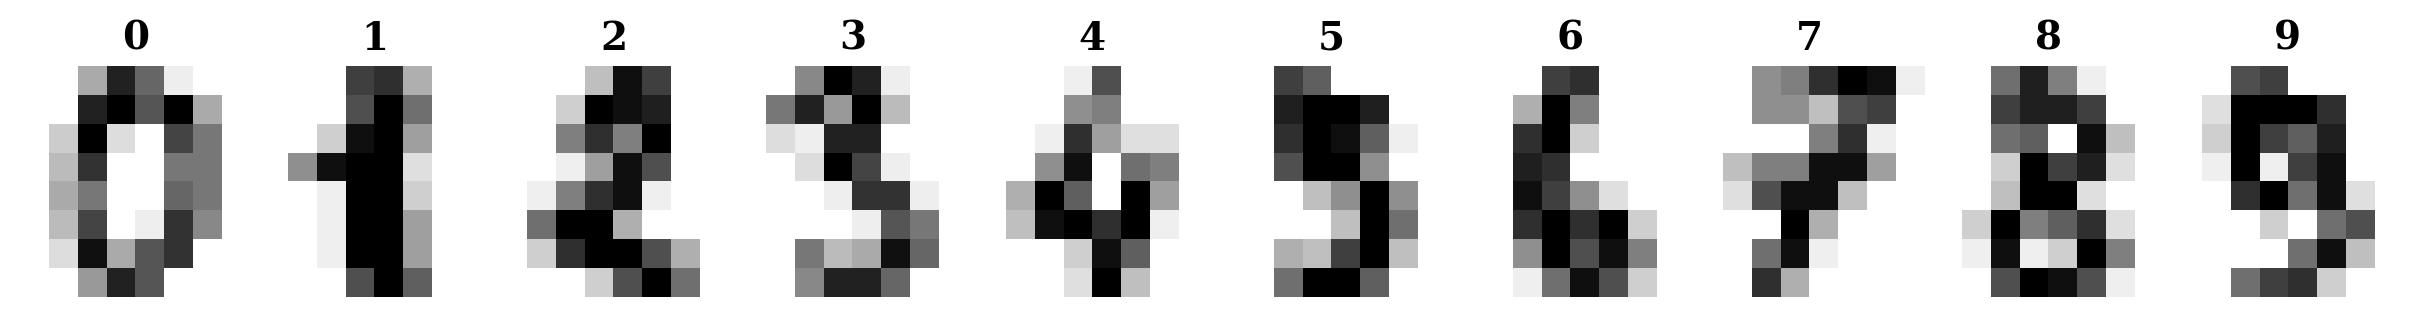
\includegraphics[width=0.42\textwidth]{visual_mnist_samples.png}
\end{column}
\end{columns}
\end{frame}

\begin{frame}{A9a --- Logistic Loss (Convex)}
\centering
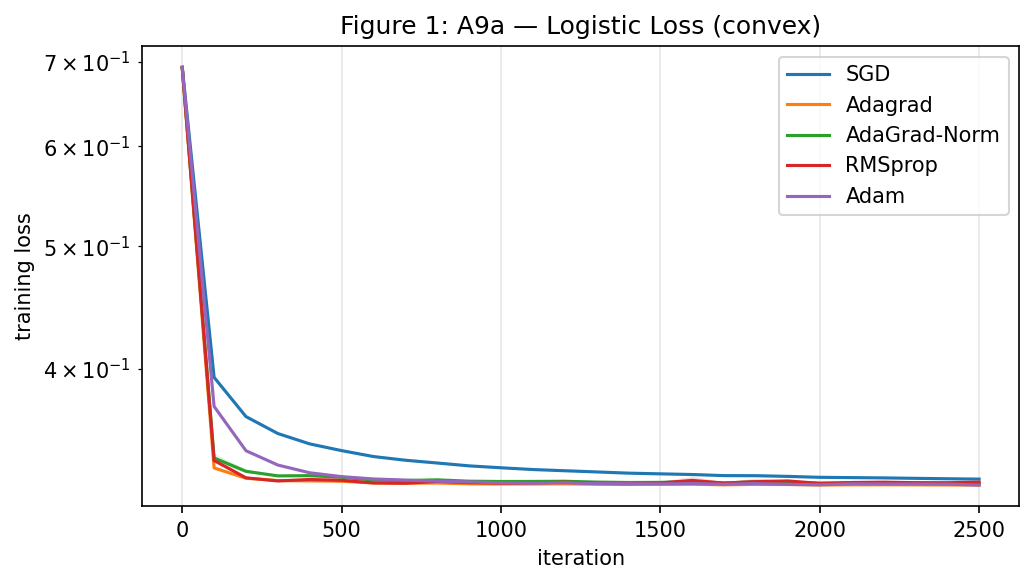
\includegraphics[width=0.48\textwidth]{fig01_a9a__logistic_loss_(convex).png}%
\hfill
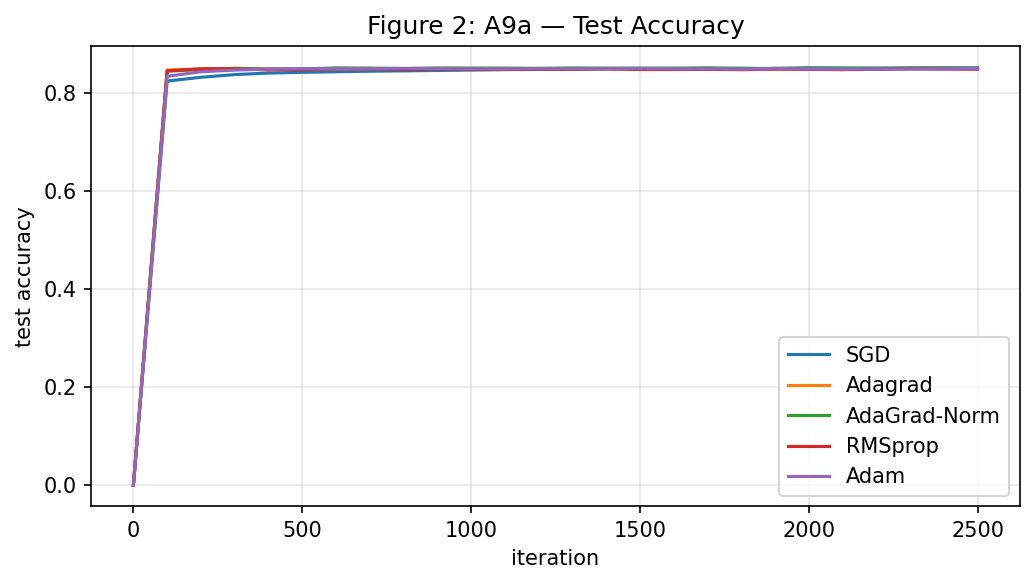
\includegraphics[width=0.48\textwidth]{fig02_a9a__test_accuracy.png}

\vskip0.3cm
\small
RMSprop \& Adagrad converge fastest; all reach $\approx 85\%$ test accuracy.
\end{frame}

\begin{frame}{MNIST --- Softmax Cross-Entropy}
\centering
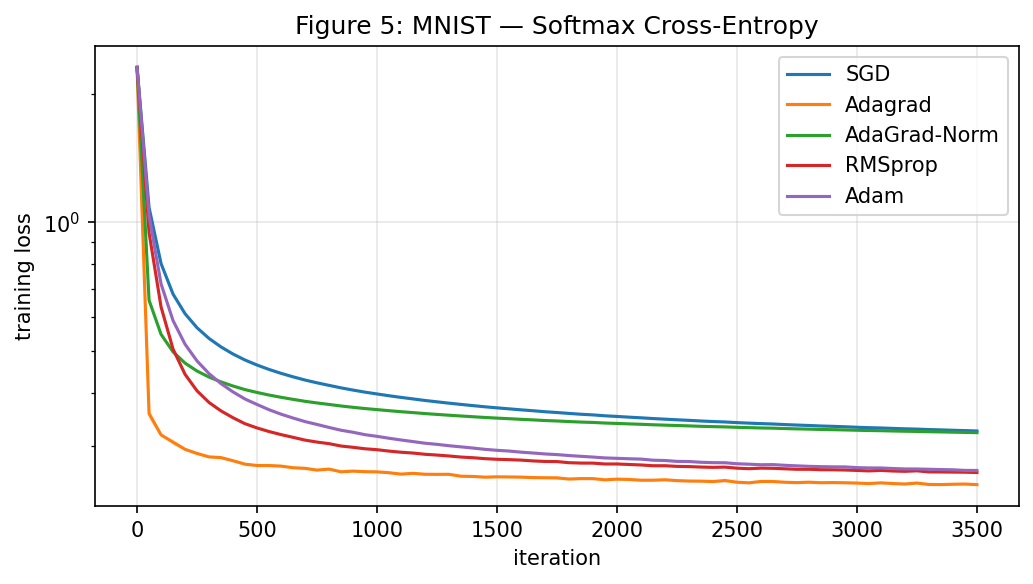
\includegraphics[width=0.48\textwidth]{fig05_mnist__softmax_cross-entropy.png}%
\hfill
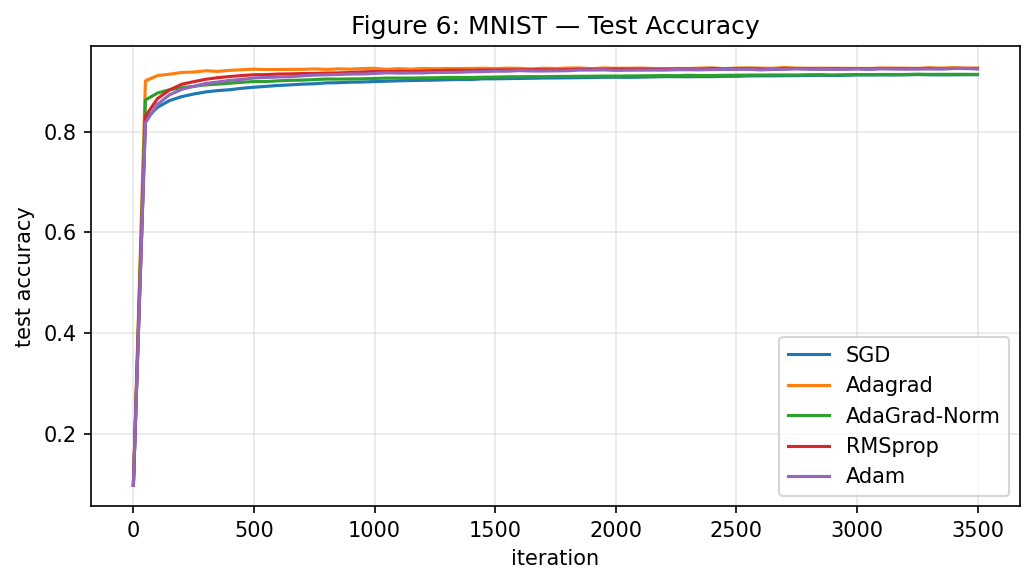
\includegraphics[width=0.48\textwidth]{fig06_mnist__test_accuracy.png}

\vskip0.3cm
\small
Adagrad dominates; RMSprop \& Adam close behind.\\
SGD needs $3\times$ more iterations to match.
\end{frame}

\begin{frame}{Key Takeaways \& Outlook}
\begin{itemize}
  \setlength{\itemsep}{0.4cm}
  \item Adaptive methods converge \textbf{significantly faster} in early iterations
  \item \textbf{RMSprop} is surprisingly effective --- fast forgetting helps
  \item Final accuracy differences are small on these tasks\\
        $\to$ adaptive methods shine in \textbf{speed}, not final quality
  \item Non-convex regularizer has limited impact at moderate $\lambda$
\end{itemize}
\vskip0.3cm
\textbf{Remaining for the report:}\\
{\small Learning rate sweeps $\cdot$ wall-clock comparison $\cdot$ larger $\lambda$ analysis $\cdot$ NeurIPS format (deadline 21.07)}
\end{frame}

\begin{frame}{References}
\small
\begin{itemize}
  \setlength{\itemsep}{0.25cm}
  \item Kingma, D.\ \& Ba, J.\ (2014). \textit{Adam: A method for stochastic optimization.} arXiv:1412.6980
  \item Duchi, J., Hazan, E.\ \& Singer, Y.\ (2011). \textit{Adaptive subgradient methods for online learning and stochastic optimization.} JMLR 12.
  \item Ward, R., Wu, X.\ \& Bottou, L.\ (2020). \textit{AdaGrad stepsizes: Sharp convergence over nonconvex landscapes.} JMLR 21.
  \item Tieleman, T.\ \& Hinton, G.\ (2012). \textit{Lecture 6.5 --- RMSprop.} Coursera Neural Networks for ML.
  \item Reddi, S.\ et al.\ (2018). \textit{On the convergence of Adam and beyond.} ICLR.
  \item Xu, C.\ \& Zhang, J.\ (2001). \textit{A survey of quasi-Newton equations and quasi-Newton methods for optimization.} Annals of Operations Research 103.
\end{itemize}
\end{frame}

% ── Closing slide ─────────────────────────────────────────────────
{
\setbeamercolor{background canvas}{bg=unibaselteal}
\begin{frame}[plain,c]
  \centering
  {\usebeamerfont{title}\color{black}Thank you!\par}
  \vskip1cm
  {\large Questions?\par}
\end{frame}
}

% ==================================================================
% BACKUP SLIDES (not part of main presentation)
% ==================================================================

\appendix

{
\setbeamercolor{background canvas}{bg=unibaselteal}
\begin{frame}[plain,c]
  \centering
  {\usebeamerfont{title}\color{black}Backup Slides\par}
\end{frame}
}

\begin{frame}{Learning Rate Sensitivity}
\centering
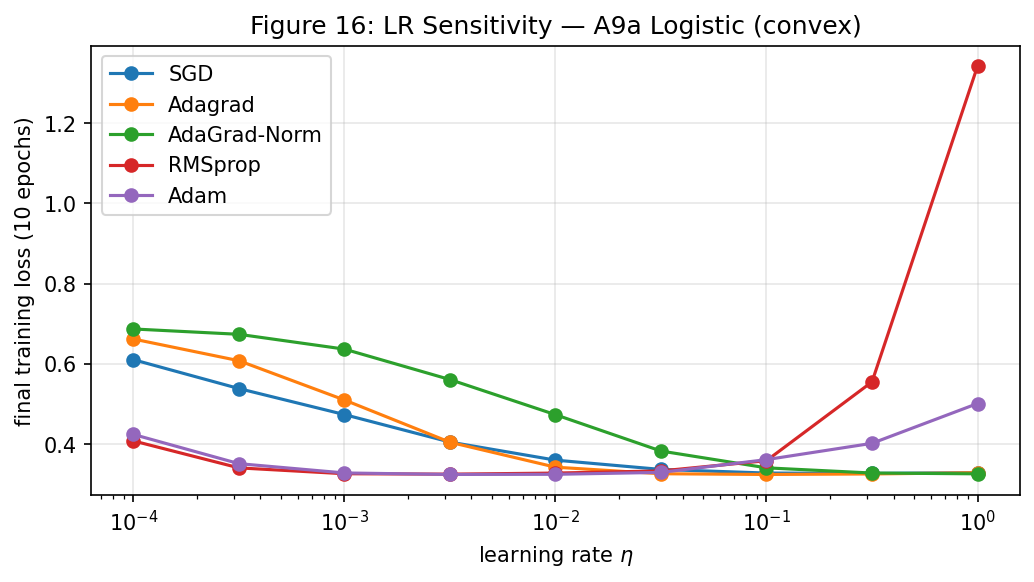
\includegraphics[width=0.75\textwidth]{fig16_lr_sweep_a9a.png}

\vskip0.3cm
\small
Adagrad \& AdaGrad-Norm are most robust to $\eta$; RMSprop diverges at large $\eta$.
\end{frame}

\begin{frame}{A9a --- Non-convex Regularizer}
\centering
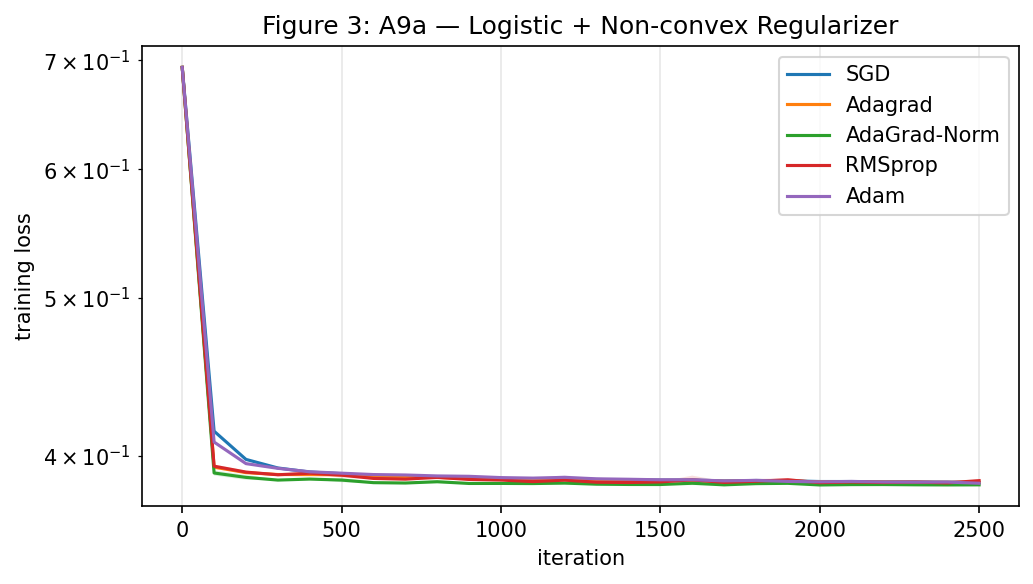
\includegraphics[width=0.48\textwidth]{fig03_a9a__logistic__non-convex_regularizer.png}%
\hfill
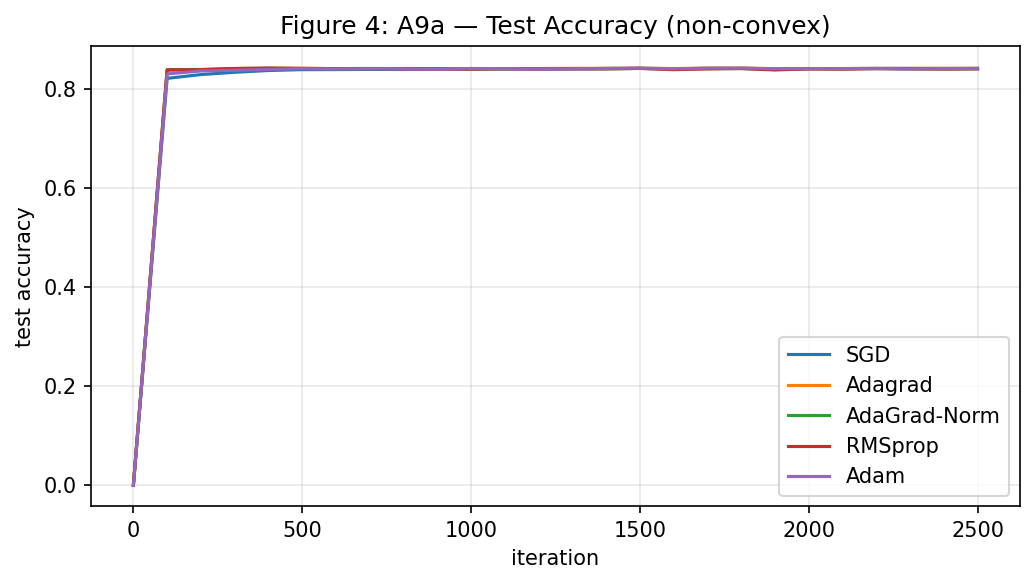
\includegraphics[width=0.48\textwidth]{fig04_a9a__test_accuracy_(non-convex).png}

\vskip0.3cm
\small
Non-convex regularizer raises final loss but ranking stays the same.\\
Accuracy is nearly identical to the convex case.
\end{frame}

\begin{frame}{Gradient Norms}
\centering
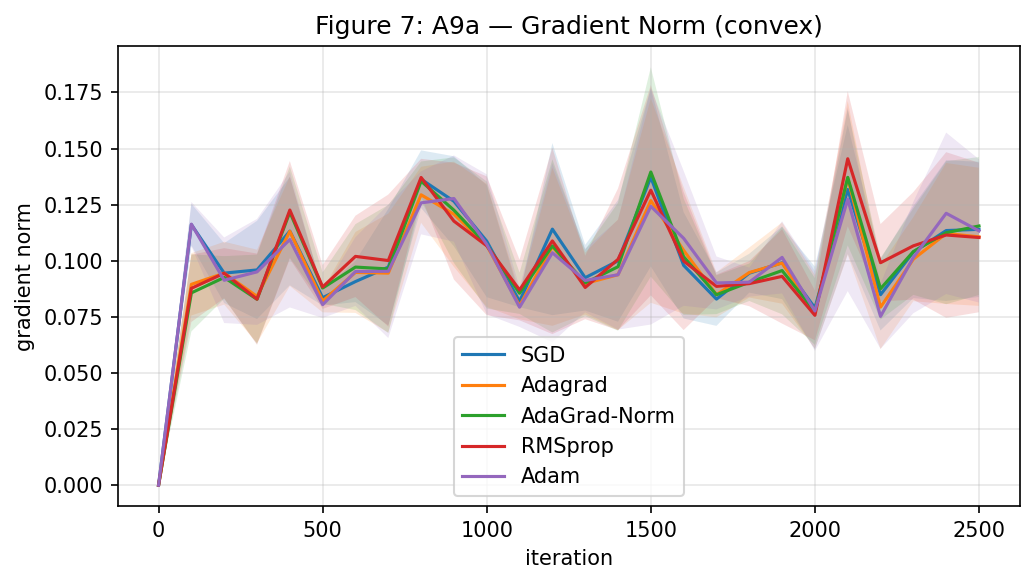
\includegraphics[width=0.32\textwidth]{fig07_a9a__gradient_norm_(convex).png}%
\hfill
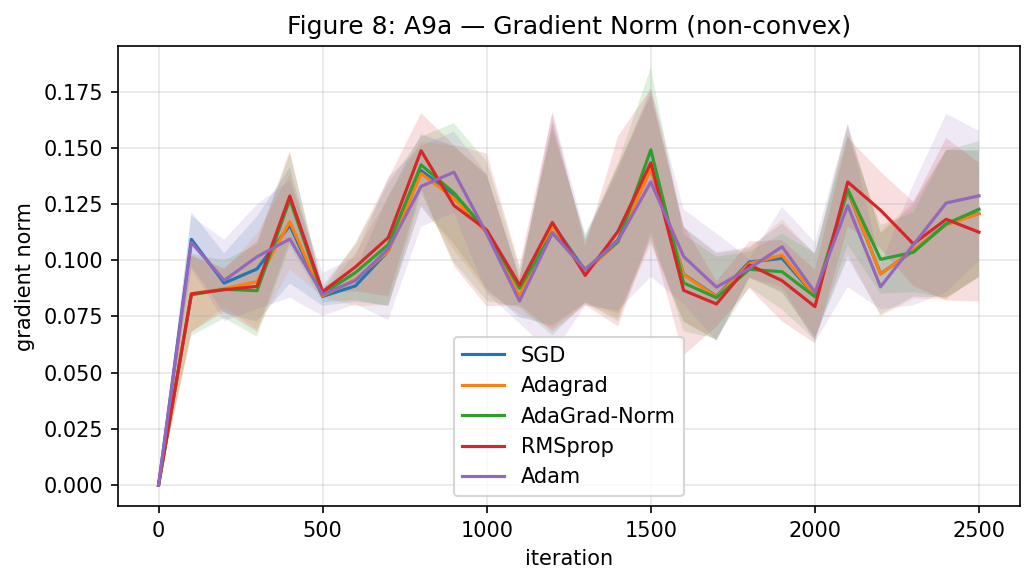
\includegraphics[width=0.32\textwidth]{fig08_a9a__gradient_norm_(non-convex).png}%
\hfill
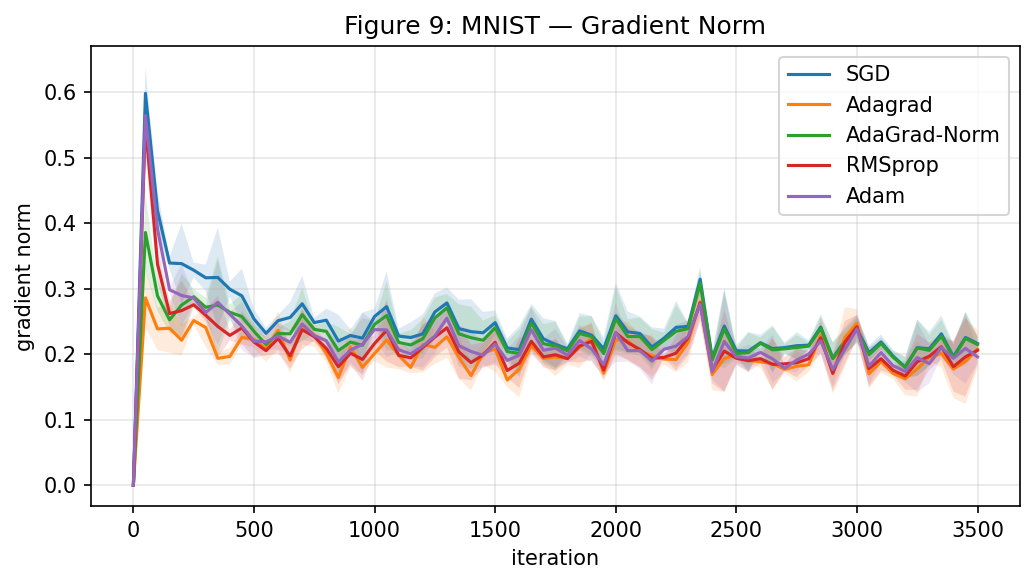
\includegraphics[width=0.32\textwidth]{fig09_mnist__gradient_norm.png}

\vskip0.3cm
\small
Gradient norms reveal \textbf{why} adaptive methods help:\\
they normalize large initial gradients, preventing overshooting.
\end{frame}

\begin{frame}{Summary of Results}
\centering
\small
\begin{tabular}{@{}l r r r r r r@{}}
\toprule
& \multicolumn{2}{c}{\textbf{A9a (convex)}} & \multicolumn{2}{c}{\textbf{A9a (non-cvx)}} & \multicolumn{2}{c}{\textbf{MNIST}} \\
\cmidrule(lr){2-3}\cmidrule(lr){4-5}\cmidrule(lr){6-7}
\textbf{Optimizer} & Loss & Acc & Loss & Acc & Loss & Acc \\
\midrule
SGD          & 0.337 & 0.847 & 0.349 & 0.847 & 0.286 & 0.923 \\
Adagrad      & 0.328 & 0.850 & 0.340 & 0.850 & 0.271 & 0.925 \\
AdaGrad-Norm & 0.333 & 0.848 & 0.344 & 0.848 & 0.302 & 0.917 \\
RMSprop      & 0.328 & 0.849 & 0.340 & 0.849 & 0.278 & 0.924 \\
Adam         & 0.330 & 0.849 & 0.341 & 0.849 & 0.276 & 0.924 \\
\bottomrule
\end{tabular}

\vskip0.5cm
\textit{Note: Exact values may vary slightly. These are averaged over 3 seeds.}
\end{frame}

\begin{frame}{Wall-Clock Time Comparison}
\centering
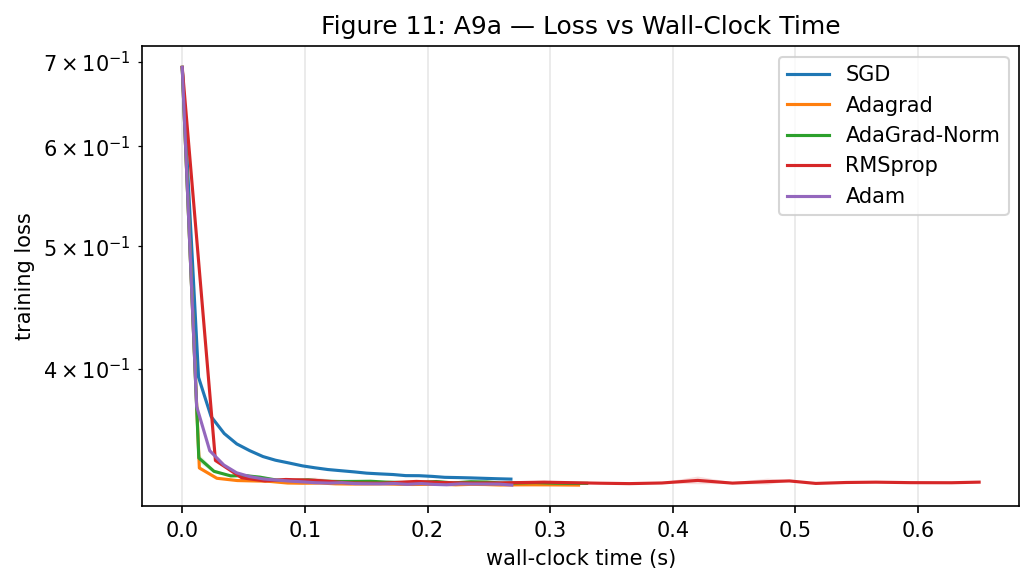
\includegraphics[width=0.48\textwidth]{fig11_wallclock_a9a_—_loss_vs_wall-clock_time.png}%
\hfill
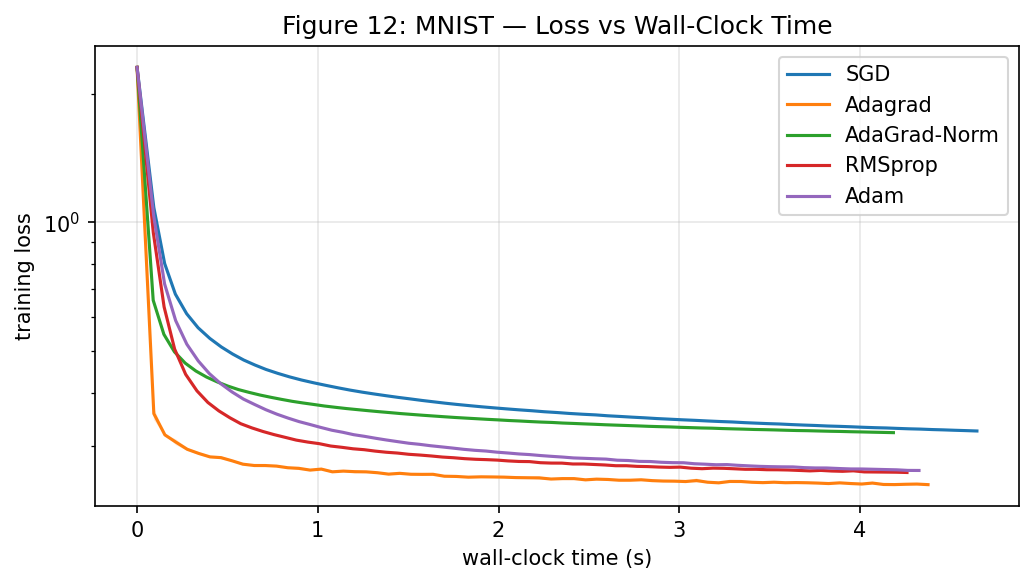
\includegraphics[width=0.48\textwidth]{fig12_wallclock_mnist_—_loss_vs_wall-clock_tim.png}

\vskip0.3cm
\small
Adaptive methods have slightly more per-step overhead, but reach low loss faster in wall-clock time.
\end{frame}

\begin{frame}{Non-convex Regularizer --- $\lambda$ Sweep}
\centering
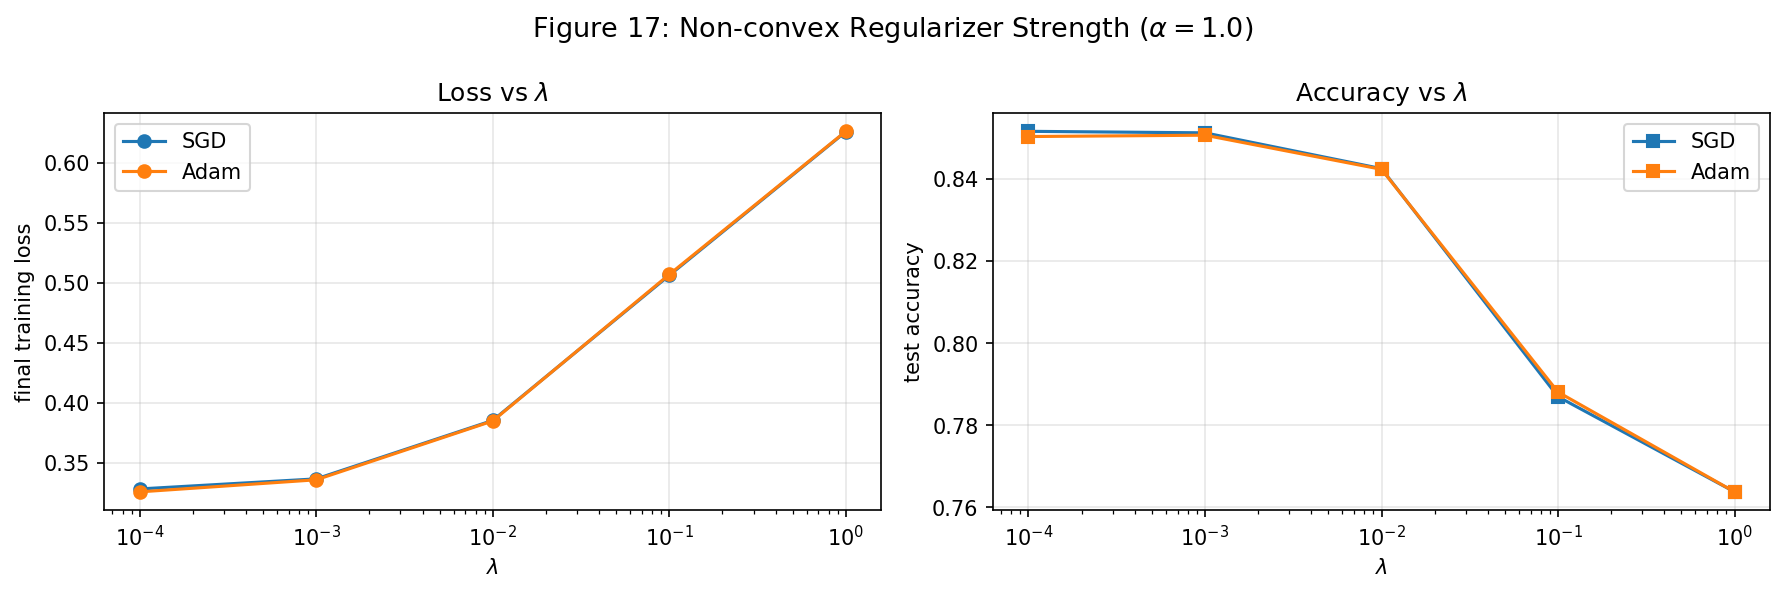
\includegraphics[width=0.75\textwidth]{fig17_lambda_sweep.png}

\vskip0.3cm
\small
At $\lambda \ge 0.1$ the regularizer dominates, pushing weights to zero and degrading accuracy.\\
Both SGD and Adam respond similarly.
\end{frame}

\begin{frame}{Empirical vs.\ Theoretical Convergence}
\centering
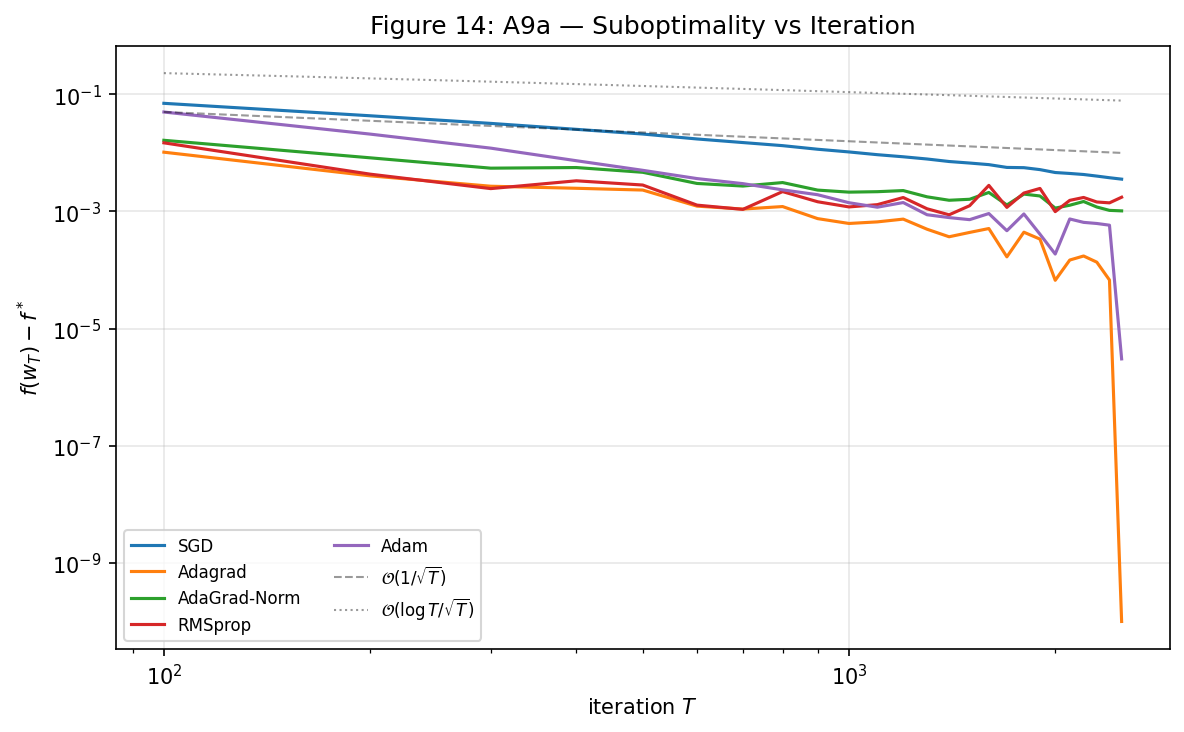
\includegraphics[width=0.48\textwidth]{fig14_convergence_rate_a9a_—_suboptimality_vs_it.png}%
\hfill
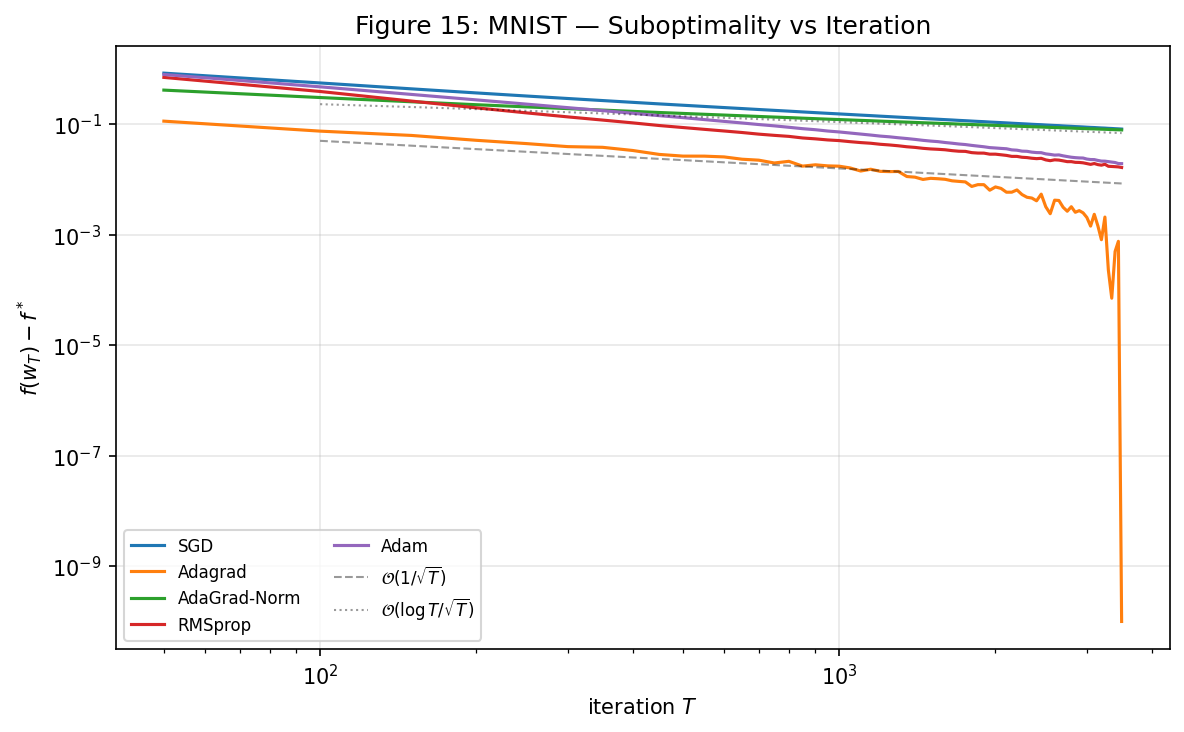
\includegraphics[width=0.48\textwidth]{fig15_convergence_rate_mnist_—_suboptimality_vs_.png}

\vskip0.3cm
\small
All methods converge faster than the worst-case $\mathcal{O}(1/\sqrt{T})$ bound.\\
Adagrad shows the steepest empirical rate on both datasets.
\end{frame}

\end{document}
